%%%%%%%%%%%%%%%%%%%%%%%%%%%%%%%%%%%%%%%%%%
\chapter{Modeling CFD-DEM} \label{sec:modeling-cfd-dem}
%%%%%%%%%%%%%%%%%%%%%%%%%%%%%%%%%%%%%%%%%%
[talk about how lacking the DEM result is without the inclusion of helium in analysis. There are some Fusion papers on conductivity in vacuum and with helium]

We now consider the influence of helium on thermal transport of deposited nuclear energy as it is carried away by the cooled structural walls. We begin by considering the fluid in a continuum sense and the pebbles in a discrete one. The interactions of the fluid and solid are characterized by effective relationships in each discretized cell of fluid. We then consider an mesoscopic approach to the fluid-solid interaction with the Lattice-Boltzmann method. 

The chapter begins with introduction of the coupled fluid dynamics - discrete element method (CFD-DEM) approach: governing equations, discretization techniques, and algorithms.

We then do LBM. And stuff.

%%%%%%%%%%%%%%%%%%%%%%%%%%%%%%%%%%%%%%%%%%
\subsection{Helium in the DEM Framework}\label{sec:cfdem-heat-transfer}

The numerical framework behind the discrete element was given in \cref{sec:particle-dynamics}. In the DEM model, each pebble obeys Newton's equations of motion. As the fluid passes through the packed bed of pebbles, it imparts a force on each individual pebble which cumulatively total to the pressure drop across the bed. To include the influence of helium, we simply augment the the linear momentum of Eq.~\ref{eq:newton-translational} to include the drag force of the fluid on the particle. The momentum balance of our Lagrangian-tracked pebble now reads,
\begin{equation}\label{eq:cfdem-dem-momentum}
	m_i  \ddt{\vec{r}_i} = m_i\vec{g} + \vec{f}_i + \beta_i V_i \Delta \vec{u}_{if}
\end{equation}
where all but the last term is identical to Eq.~\ref{eq:newton-translational} but the last term accounts for the fluid. $\Delta \vec{u}_{if} = \vec{u}_f - u_i$, is the relative velocity between the fluid and pebble, $i$, and the inter-phase momentum exchange coefficient, $\beta_i$, acts upon the entire pebble volume, $V_i$. 

Similarly, as the helium of temperature $T_f$ passes over the particle at temperature $T_i$, energy will be exchanged. For consistency with the momentum equation, we introduce an inter-phase energy exchange coefficient (a renaming of the heat transfer coefficient) which we assume to be constant for the entire surface of the particle. The energy balance of the particle was given in Eq.~\ref{eq:thermoFirstLaw}. After adding the inter-phase energy exchange coefficient, it now reads,
\begin{equation}\label{eq:cfdem-dem-energy}
	m_iC_i \ddt{T_i} = Q_{s,i} + \sum_{j=1}^Z Q_{ij} + \beta_{E,i} A_i \Delta T_{if}
\end{equation}
where again we have only needed to add the last term to account for the energy deposited/removed by the fluid. $\Delta T_{if} = T_f - T_i$, and the inter-phase energy exchange coefficient, $\beta_{E,i}$, acts upon the pebble surface area, $A_i$.

These simple additions to the governing equations of momentum and energy of each particle are all that are necessary to introduce helium into the DEM computations. The difficulty arises in the computation of the inter-phase exchange coefficients, $\beta_i$ and $\beta_{E,i}$. We will discuss their calculations next.

\subsection{Inter-phase Exchange Coefficients}
In \cref{sec:modeling-pressure-drop}, we showed a number of correlations that engineers use to calculate the pressure drop in packed beds of spheres. The purge gas in ceramic breeders is meant to travel at very low flow rates to maximize the absorption of tritium. Furthermore, the pebble beds will always be near the close-packed limit. As such, the particle Reynolds number for these flows is often near unity and the Kozeny-Carman equation as applicable for Stokes flow is quite sufficient (see the assumptions leading to Eq.~\ref{eq:K-C-non-dim}). However, the Koch-Hill-Ladd correlation of Eq.~\ref{eq:khl-correlation} which includes terms for both the Stokes flow correlation (as a function of $\phi$) in the zero-Reynolds number limit and the viscous effects with a Reynolds number-dependent term is a general correlation that reduces to the Kozeny-Carman correlation in the close-packed, zero-Reynolds number limits. Thus for our model, we implement the KHL correlation.

The inter-phase momentum exchange coefficient is simply a re-writing of the non-dimensional drag force from Eq.~\ref{eq:khl-correlation}. The common form by Gidaspow\cite{gidaspow1994multiphase} differs from what we use here by a factor of $1-\phi$ due to definitions of the drag force. We use the form from Koch, Hill, \& Ladd.\cite{Hoef2005,Benyahia2006}
\begin{equation}\label{eq:interphase-momentum}
	\beta_{i} = \frac{18\mu_f}{d_{p,i}^2}(1-\phi_k)\phi_k F
\end{equation}
where $\mu_f$ is the fluid viscosity and the diameter of pebble $i$ is $d_{p,i}$. The packing fraction, $\phi_k$, in this equation is the local packing fraction in the fluid cell $k$. This value will differ from the global/bulk value in near-wall regions. Container walls have long been known to theoretically and experimentally force order to the packing regardless of shape of packing.\cite{Hunt1990,Benenati1962,Baird1958} For example, the void fraction ($\epsilon = 1-\phi$) in narrow annular containers using the correlation from Mueller, as a function of wall-distance in a cylinder is,\cite{Mueller1999}
\[
\epsilon = \epsilon_0 + (1-\epsilon_0)J_0(ar^*)e^{-br^*}
\]
where $r^*$ is the non-dimensional distance from the wall; here it is defined in terms of the pebble diameter, $r^* = r/d_p$. The constants, a and b, are defined in terms of the size parameter $\alpha = D/d_p$ where $D$ is the diameter of the annular tube. First, $a$ is
\[
    a= 
\begin{cases}
    7.383 - \cfrac{2.932}{\alpha - 9.864}, & \text{if }\  \alpha \geq 13\\
    8.243 - \cfrac{12.98}{\alpha + 3.156}, & \text{if} \ 13 \geq \alpha \geq 2.61
\end{cases}
\]
then
\[
b = 0.304 - \cfrac{0.724}{\alpha}
\]
The bulk void fraction is found from the correlation:
\[
\epsilon_0 = 0.379 + \cfrac{0.078}{\alpha - 1.8}
\]

We then plot the packing fraction as a function of distance from the container wall for two example sizes, diameters of 20$d_p$ and 5$d_p$, in Fig.~\ref{fig:packingDist}. This example is meant to demonstrate the varying packing fraction in a packed bed that is described with a bulk or global packing fraction. The size of the discretized cell relative to the pebble will dictate how much of the void fraction variation is captured in the volume-averaged equations.

\begin{figure}[htbp]
\begin{center}
	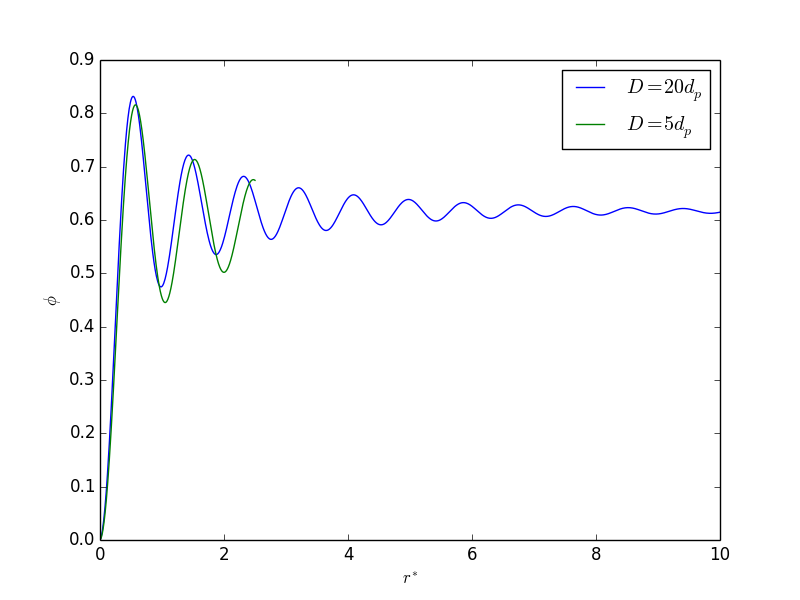
\includegraphics[width = \singleimagewidth]{chapters/figures/annular-packing-fraction.png}
	\caption{Showing the packing fraction approach the bulk value after a few pebble diameters when the pipe is 20$d_p$ and that when the pipe is only 5$d_p$, the packing fraction at any radius is not the same as the bed average.}
	\label{fig:packingDist}
\end{center}
\end{figure}
\FloatBarrier


The inter-phase energy transfer coefficient is of the same form as a traditional heat transfer coefficient and is likewise calculated from the Nusselt number for the helium flow.
\begin{equation}\label{eq:interphase-energy}
	\beta_{E,i} = \frac{\Nu k_f}{d_{p,i}}
\end{equation}
where $k_f$ is the thermal conductivity of the fluid. Several correlations for determining the Nusselt number were given in \cref{sec:particle-convection}. We opt for the correlation provided by Li \& Mason.\cite{Li2000} Which is applicable to a wide range of Reynolds number flows [and packing fractions?].

From Eqs.~\ref{eq:interphase-momentum} and~\ref{eq:interphase-energy}, we have a formulation wherein knowledge of the flow field around our pebbles will allow calculation of dimensionless drag, $F$, and Nusselt number, $\Nu$, and the flow is coupled to our DEM computations with simple additions to the equations of motion and energy of the pebble. We next 




\subsection{Volume-averaged Thermofluid Flow}

The gas phase flow field will be treated in a method analogous to the approach of volume-averaging theory (VAT).\cite{Sbutega2013,whitaker1999method,Tsuji1992} The VAT allows treatment of complex porous flows with smooth continuous equations. In the VAT, we average over a discrete space to replace complex geometry with a fictitious, smooth, continuous medium in which quantities of interested are defined independently of whether specific locations in that space are, for instance, solid or gas.

In this formulation of the gas flow, we discretize the gas space with cells that are much larger than the individual particles; in the application of our CFD-DEM coupling, this meant approximately 5~6 particles per cell. With VAT, the particles themselves are not resolved in the fluid space but are simply introduced via closure terms.\cite{Sbutega2013,Horvat2006} Derivation of the governing equations of VAT can be found in Sbutega \& Catton\cite{Sbutega2013}. The momentum and energy of a fluid flow through a solid phase with volume-averaged Navier-Stokes and energy equations are applied to each cell, $k$, in the discretized fluid space,
\begin{subequations}\label{eq:cfd-equations}
\begin{align}
\pder[\epsilon_k \rho_f]{t} + \nabla\cdot(\epsilon_k \vec{u}_f \rho_f) &= 0\\
\pder[\epsilon_k \vec{u}_f]{t} + \nabla\cdot(\epsilon_k \vec{u}_f \vec{u}_f) &= -\frac{\epsilon_k}{\rho_f}\nabla P_f + \nabla\cdot\left(\nu_f\epsilon_k\nabla \vec{u}_f\right) - \frac{S_k}{\rho_f}\\
\pder[\epsilon_k T_f]{t} + \nabla\cdot(\epsilon_k \vec{u}_f T_f) &= \nabla\left(\epsilon_k\nabla T_f\right)-\frac{E_k}{\rho_fC_f}
\end{align}
\end{subequations}

The packing fraction in any fluid cell is calculated by summing through all the volumes of particles located in cell $k$,
\begin{equation}
	\phi_k = \frac{1}{V_k}\sum_{\forall i \in k} V_{p,i}
\end{equation}
where the fluid void fraction is the complement of the solid packing fraction, $\epsilon = 1 - \phi$. 

Coupling the fluid phase to the particles happens with the sink terms in momentum and energy of $S_k$ and $E_k$, respectively. They are volume-weighted sums of the drag forces and energy exchanges, respectively, for all particles in the discretized fluid cell,
\begin{subequations}\label{eq:cfd-sources}
\begin{align}
	S_k &= \frac{1}{V_k}\sum_{\forall i \in k} \beta_i V_i \Delta \vec{u}_{if} \label{eq:cfd-mom-source}\\
	E_k &= \frac{1}{V_k}\sum_{\forall i \in k} \beta_{E,i} A_i \Delta T_{if}
\end{align}
\end{subequations}
The inter-phase momentum and energy exchange coefficients act as the communicators between the particle information from the DEM solver and the fluid fields from CFD. Thus the motion and energy of the fluid field are intimately coupled with the particle positions and energy, but computational time is preserved by only considering volume-averaged values in the fluid domain. %The cross-communication between fluid and solid is accomplished with a coupling routine that is explained in detail in Refs. 11, 12.





\subsection{Lagrangian-Eulerian Mapping Calculations of Porosity}\label{sec:lag-eul-mapping}
\begin{figure}[t]
	\centering
	\caption{The dashed line represents a computational cell in which exist many particles. The particles with centroids inside the cell are shaded red.}
	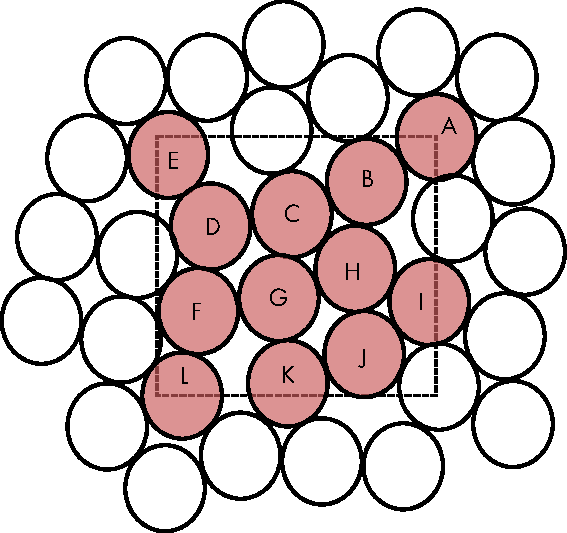
\includegraphics[width=\singleimagewidth]{chapters/figures/void-fraction-cell.pdf}\label{fig:centroid-void-fraction}
\end{figure}
The simplest method for calculating the porosity of a CFD computational cell is to map all the DEM particles into the Eulerian volume via their centroid. We refer to this simple technique as the particle centroid method; in spite of its simplicity it is often used for large cell-to-particle volume ratios.\cite{Xu1997} A two-dimensional demonstration of the centroid technique is given in Fig.~\ref{fig:centroid-void-fraction}. In this figure, we see a computational cell (dashed line) in which many particles exist either partially or fully. The particles shaded in red have their centers located inside the cell and therefore have their entire volume contribute to the calculation of the porosity. The porosity is calculated as
\begin{equation}
	\epsilon_\text{cell} = 1-\frac{1}{V_\text{cell}}\sum_{i = A}^{i=L}V_{p,i}
\end{equation}
where $V_{p,i}$ is the volume of particle $i$. As the cell size begins to approach the size of the particle, erroneous calculations of porosity arise. This is visible, for instance, by particle A in Fig.~\ref{fig:centroid-void-fraction}. This particle has only a quarter of its volume inside the cell but the porosity of the cell is computed as if the entire particle existed inside. Hoomans\etal~recognized this limitation of the centroid method and introduced a fractional volume method.\cite{Hoomans1996} The porosity is found as
\begin{equation}
	\epsilon_\text{cell} = 1-\frac{1}{V_\text{cell}}\sum_{i = A}^{i=L}f_iV_{p,i}
\end{equation}
where $f_i$ is the fraction of the particle in the Eulerian cell. A similar approach taken by Kloss\etal~ and Zhao \& Shan is the divided technique.\cite{Kloss2012,Zhao2013a} In this technique, the spherical particle is artificially divided into a number of regions with markers indicating their location. For example, see now how particle A is treated in Fig.~\ref{fig:centroid-void-fraction-divided}. Instead of searching for centroids of particles, each particle has a search through the marker points (the black dots drawn in Pebble A) and the volume of that section of the sphere is assigned to whichever cell it falls inside. 
\begin{figure}[t]
	\centering
	\caption{The dashed line represents a computational cell in which exist many particles. The particles with centroids inside the cell are shaded red.}
	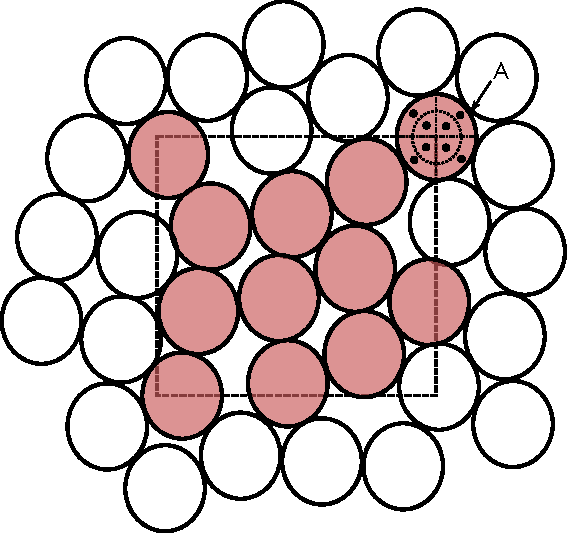
\includegraphics[width=\singleimagewidth]{chapters/figures/void-fraction-divided-cell.pdf}\label{fig:centroid-void-fraction-divided}
\end{figure}

As the computational cell volume approaches the size of a single particle $V_\text{cell}\rightarrow V_p$, the centroid and divided techniques break down. A technique introduced by Link\etal~treats the particle as a porous cube and allows computations when a cell is completely occupied by only a single particle.\cite{Link2005} Peng\etal~offer an an analytic technique as well as guidelines for validity of either analytic or centroid techniques.\cite{Peng2014} In this work, we will always apply the divided technique of Kloss\etal~based on the geometry of our packed bed flow and the guidelines established by Peng\etal.\cite{Kloss2012,Peng2014}


\subsection{Eulerian-Lagrangian Mapping Calculations of Force and Energy}
Once the fluid momentum and energy fields are calculated in the Eulerian grid, the coupled inter-phase exchange coefficients must map the velocities and temperatures onto the particles in the Lagrangian DEM framework. A particle centroid method is always used in the exchange onto the particles. Referencing Fig.~\ref{fig:centroid-void-fraction}, the velocity and temperature of the dashed cell is mapped only onto the particles highlighted in red. The approach has been used successfully by others.\cite{Xu1997,Link2005,Kloss2012}







\section{Discussion of CFD-DEM Governing Equations}
Early work on gas-particle flow models treated the solid and gas phases as two inter-penetrating continuum. The solid and gas were treated with the so-called two fluid model (TFM) by Anderson \& Jackson in 1967.\cite{Anderson1967} The TFM approach is similar to the VAT approach in that the fluid computational cell is sufficiently large to include many individual particles but still smaller than the size of the system.\cite{Enwald1996} The governing equations of TFM are fundamentally similar to Eqs.~\ref{eq:cfd-equations} but required constitutive equations for closure between the fluid and solid phases. Zhou\etal~show the equivalence of the governing equations of TFM and CFD-DEM.\cite{Zhou2010} The essential difference is that the issue of closure is removed with the information from DEM providing direct coupling to the fluid phase.

Since the introduction of the CFD-DEM coupling methodology by Tsuji\etal~in 1993 and then Hoomans\etal~in 1996, many researchers have adopted the approach when particle-scale information of granular and fluidized beds is important.\cite{Tsuji1993,Hoomans1996} Fluidized beds have many industrial applications and are most often studied with coupled CFD-DEM tools. A short example of work can be found in Refs.~\cite{Xu1997,Patankar2001,Swasdisevi2005,Deen2007,Zhang2008,Chu2008,VanBuijtenen2011,Gruber2012,Peng2014}

Noting the growth in application of CFD-DEM, a systematic review of the theoretical developments behind different particular system models was given by Zhu\etal. In the chemical engineering textbook of Gidaspow, two formulations of the governing equations (labeled as Model A and Model B) are noted.\cite{gidaspow1994multiphase} Both of these models have been implemented somewhat interchangeably in CFD-DEM simulations. As pointed out by Zhu\etal, the two models differ by their treatment of the pressure drop. In Model A, the pressure drop on the system is jointly shared by the gas and solid phases. In Model B, it is only the gas phase which directly experiences the effects of pressure drop. Therefore, the two models have different forms of coupling source term, $S_k$ (see Eq.~\ref{eq:cfd-mom-source}). The source of Model B is related to that of Model A as $S_k^B = S_k^A/\epsilon - \rho_f\phi g$.

However, as is shown by Zhou\etal, there is a built-in assumption to Model B which is typically overlooked in the implementation of CFD-DEM. For an accelerating fluid, there is an added-mass in the momentum equation. In the derivation of Model B, it is tacitly assumed that the fluid is steady which is not generally valid.\cite{Zhou2010} Nevertheless, the proliferation of Model B is due to the ease in numerical implementation and, except for some situations, Model B is numerically similar to Model A for most cases studied in CFD-DEM simulations.\cite{Zhou2010} In the simulations of packed beds for tritium breeding, we choose to implement Model B as it is valid for any of the flow scenarios ever experienced by the ceramic pebble bed.







% Stability
% viscous momentum does not propagate approximately more than one cell in a single timestep. If a characteristic time, $T$, is resolved with $M$ steps, then a fluid packet will travel a distance of $L$ at velocity $U$, $TU = L$. 

%%%%%%%%%%%%%%%%%%%%%%%%%%%%%%%%%%%%%%%%%%